% Spark refernce architectures
% Copyright (C) 2016 Jan Machacek
%
% This program is free software: you can redistribute it and/or modify
% it under the terms of the GNU General Public License as published by
% the Free Software Foundation, either version 3 of the License, or
% (at your option) any later version.
%
% This program is distributed in the hope that it will be useful,
% but WITHOUT ANY WARRANTY; without even the implied warranty of
% MERCHANTABILITY or FITNESS FOR A PARTICULAR PURPOSE.  See the
% GNU General Public License for more details.
%
% You should have received a copy of the GNU General Public License
% along with this program.  If not, see <http://www.gnu.org/licenses/>.
%

%%%%%%%%%%%%%%%%%%%%%%%%%%%%%%%%%%%%%%%%%%%%%%%%%%%%%%%%%%%%%%%%%%%%%%%%%%%%%%%%
%2345678901234567890123456789012345678901234567890123456789012345678901234567890
%        1         2         3         4         5         6         7         8

\documentclass[a4paper, 10 pt, conference]{IEEEtran}

\usepackage{graphicx}
\usepackage{interval}
\usepackage{listings}
\usepackage{hyperref}

\intervalconfig {
soft open fences ,
separator symbol =; ,
}

\title{Spark Reference Architecture \\ Sensor batch processing}

\author{Jan Machacek%$^{1}$% <-this % stops a space
%\thanks{Supported by Cake Solutions Limited}% <-this % stops a space
%\thanks{$^{1}$J. Machacek is the CTO at Cake Solutions, Houldsworth Mill, Houldsworth Street, Reddish, SK5 6DA, UK {\tt\small janm at cakesolutions.net}}%
}


\begin{document}

\maketitle
\thispagestyle{empty}
\pagestyle{empty}

%%%%%%%%%%%%%%%%%%%%%%%%%%%%%%%%%%%%%%%%%%%%%%%%%%%%%%%%%%%%%%%%%%%%%%%%%%%%%%%%
\begin{abstract}

TODO

\end{abstract}


%%%%%%%%%%%%%%%%%%%%%%%%%%%%%%%%%%%%%%%%%%%%%%%%%%%%%%%%%%%%%%%%%%%%%%%%%%%%%%%%
\section{Introduction}

TODO

\section{Reference implementation}

This architecture was used in a connected fitness application. The application processes inputs from one or more sensors (smartwatch, HR sensor, smart clothes) to track fitness regimes and to deliver targeted health and fitness advice to the users. 

The application on the user's smartphone connects data from the available sensors, combines it with a statistical model of the user's behaviour, and---where available---fine-grained location services. These three inputs allow the application to make the first distinction: exercise vs. no-exercise. From the user's perspective, the system is an automated fitness trainer; from a data scientist's perspective, the biometric data the system collects allows for detailed analysis of exercises, exercise regimes, impact of exercise on the users' well-being, automated physiotherapy, and many other applications.

\subsection{Main components}

\begin{figure}[hb]
	\begin{center}
		\caption{Components}
		\label{fig:components}
		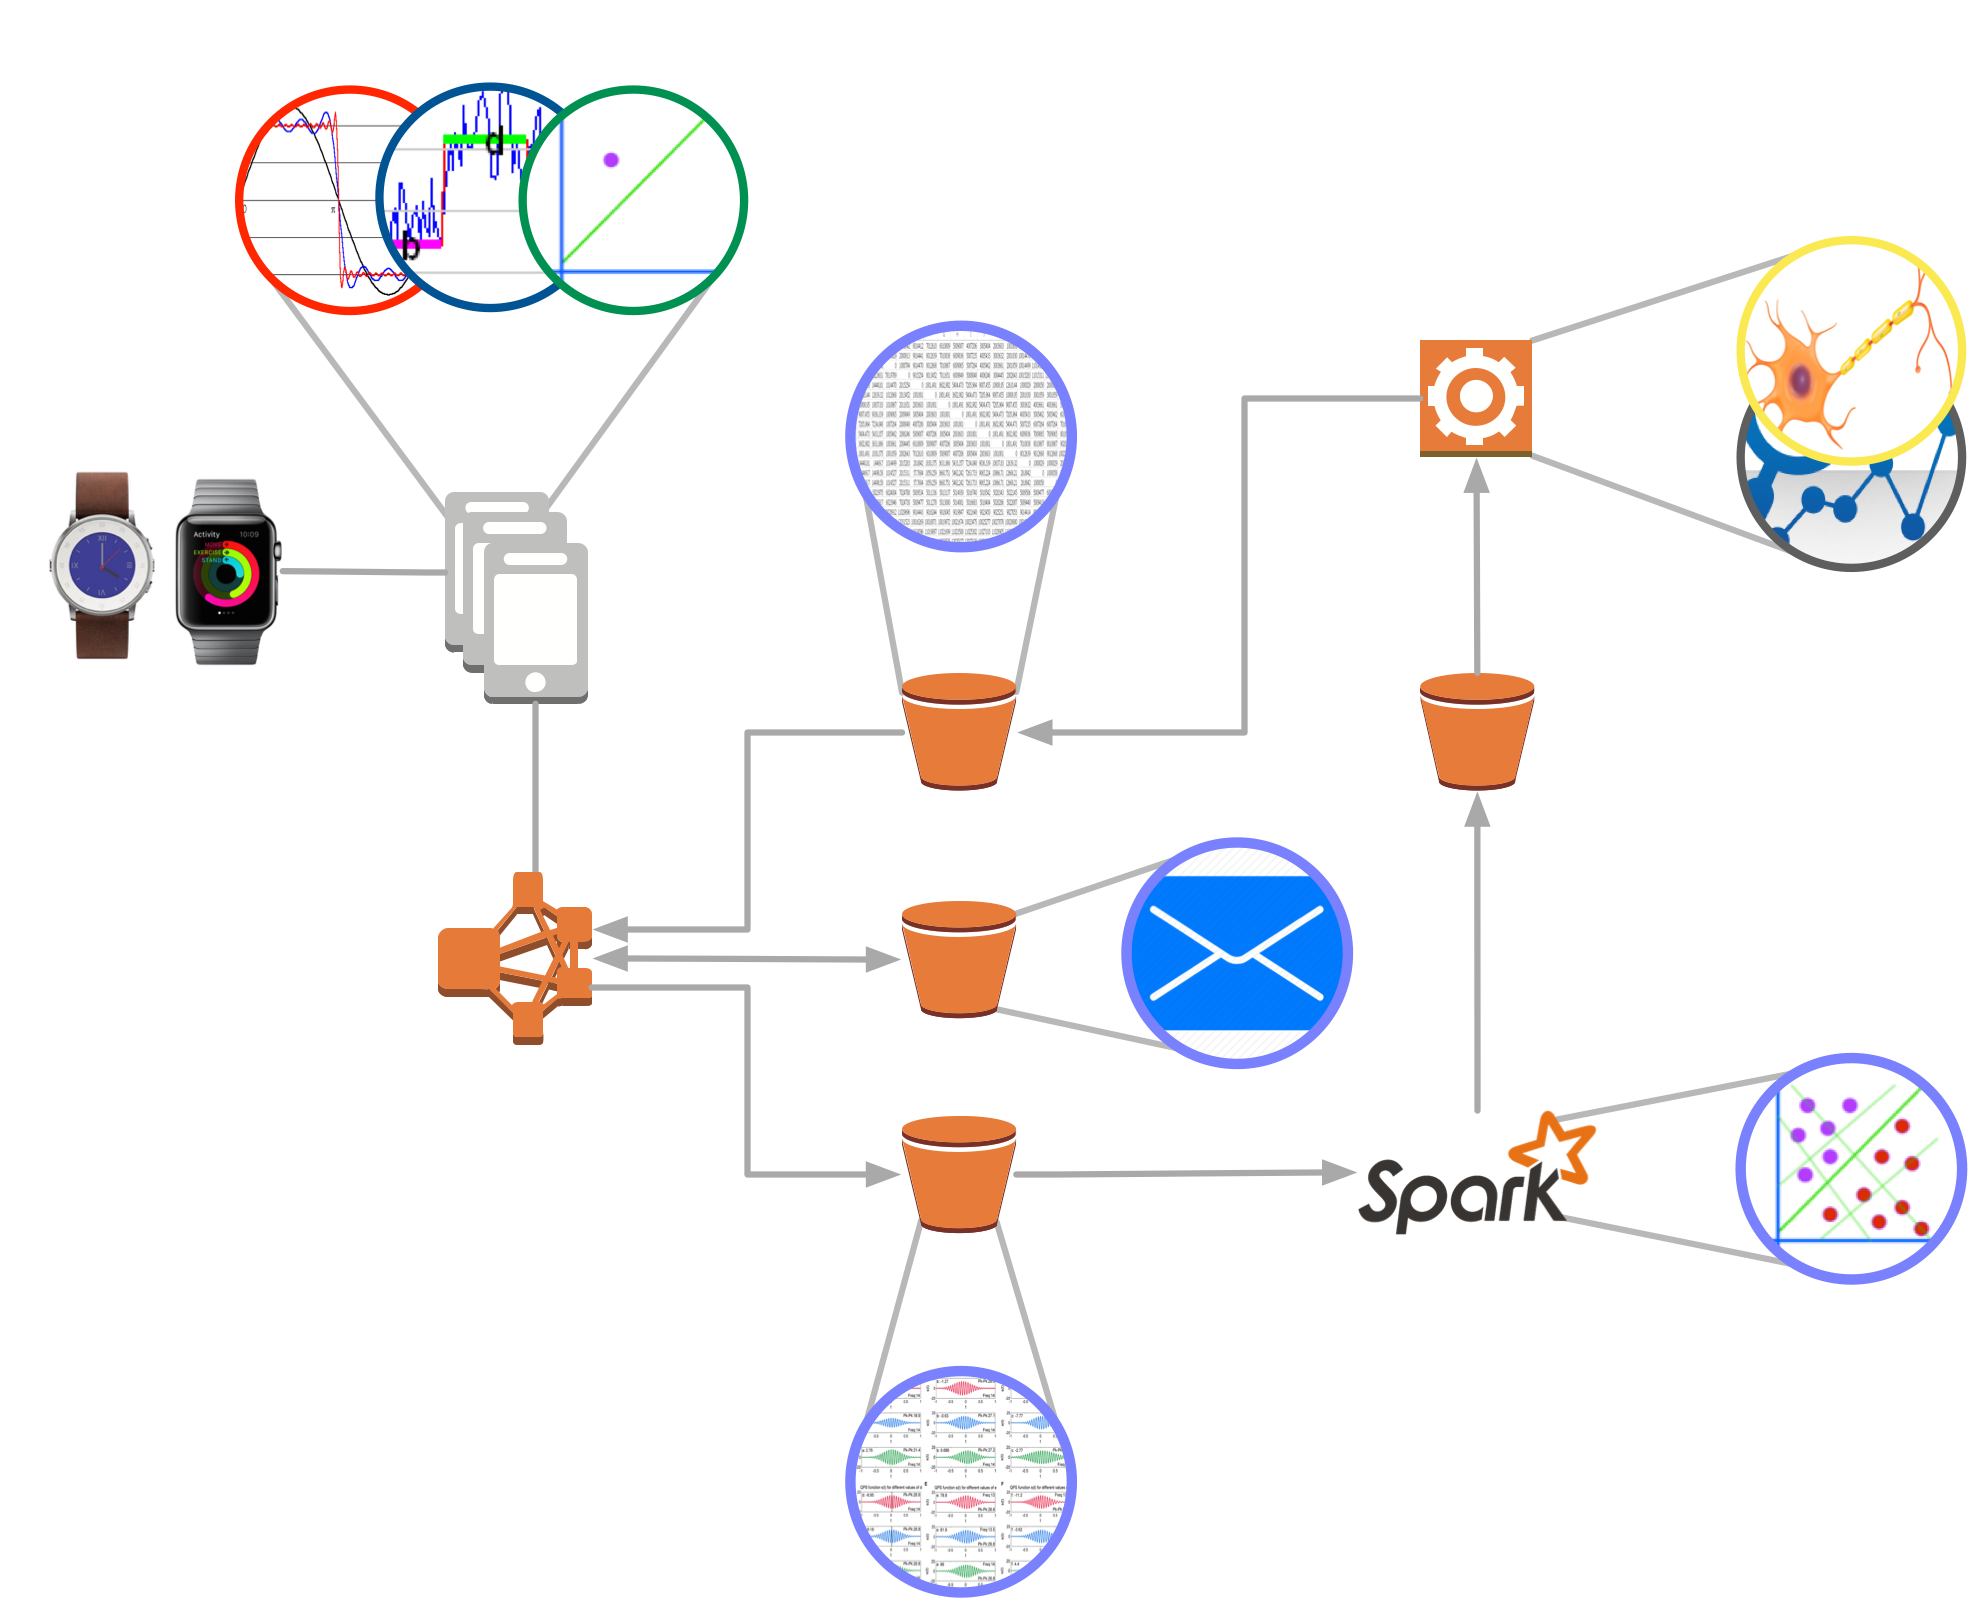
\includegraphics[width=7cm,keepaspectratio]{ri-arch.png}
	\end{center}
\end{figure}

The sensors shown here as consumer-grade wearables perform only the basic hardware interaction: there is no pre-processing of the recorded data. The system accepts accelerometer, gyroscope, heart rate and---where available---data from strain gauges in smart clothes. The mobile application performs the real-time processing of the inputs, displays the next exercise the user should perform (allowing the user to change the suggestion by simply walking to a station for a different exercise, or by beginning a different exercise). The mobile application also prompts the user to confirm correct labels for the recorded data. \emph{This is the key component in the entire system: the frictionless user experience gives the system very accurate labels on very clean data}.

The mobile submits the entire session data (the sensor data, matching labels and latest user behaviour models) in a single request to the Akka \cite{akka} cluster---a CQRS/ES \cite{cqrs-es} microservice implementation. The Akka cluster stores its events and snapshots in a journal, implemented by the Apache Cassandra \cite{apache-cassandra} database. Alongside the events and snapshots, which are opaque to non-Akka systems, the \texttt{exercise} microservice saves the sensor data and the matching labels in a properly formed tabular structure. This structure allows the Apache Spark \cite{apache-spark} cluster to be used for typical big data tasks.

The Spark cluster Lorem ipsum dolor sit amet, consectetur adipiscing elit. Donec magna purus, gravida et molestie a, bibendum et libero. Maecenas sed egestas erat. Suspendisse ullamcorper posuere erat, et finibus turpis tempor varius. Aenean tempus tellus sit amet arcu interdum, eu ornare nulla egestas. Nulla facilisi. Sed imperdiet urna et convallis consequat. Nullam nec ex eu leo auctor interdum eu id nunc. Fusce fermentum tempor gravida. Morbi sit amet augue a erat condimentum vulputate. Proin sed mattis lorem, viverra condimentum metus. Suspendisse luctus aliquam placerat. Donec sit amet mollis massa. Aliquam luctus dui in imperdiet accumsan. Nam nisi ligula, dapibus id interdum in, dictum efficitur ligula. Donec bibendum mollis convallis. Fusce maximus non orci quis laoreet.

The models are implemented in Lorem ipsum dolor sit amet, consectetur adipiscing elit. Donec magna purus, gravida et molestie a, bibendum et libero. Maecenas sed egestas erat. Suspendisse ullamcorper posuere erat, et finibus turpis tempor varius. Aenean tempus tellus sit amet arcu interdum, eu ornare nulla egestas. Nulla facilisi. Sed imperdiet urna et convallis consequat. Nullam nec ex eu leo auctor interdum eu id nunc. Fusce fermentum tempor gravida. Morbi sit amet augue a erat condimentum vulputate. Proin sed mattis lorem, viverra condimentum metus. Suspendisse luctus aliquam placerat. Donec sit amet mollis massa. Aliquam luctus dui in imperdiet accumsan. Nam nisi ligula, dapibus id interdum in, dictum efficitur ligula. Donec bibendum mollis convallis. Fusce maximus non orci quis laoreet.

\subsection{Mobile application}

The sensors send the data in 1s batches; the application on the mobile resamples the sampling rate to 50 Hz. (Accelerometer and gyroscope typically sample at this rate, heart rate and the strain gauges in smart clothes can be up-sampled to 50 Hz easily.) The mobile application ingests the data from the sensors and, together with a statistical model of the user's short-term behaviour, attempts to identify the movement. The models in the mobile application can make successful predictions of sequence of exercises in a session and the properties of each exercise (i.e. weight, number of repetitions, duration, intensity). The model used to predict sequence of exercise sessions and exercises within a session is a Markov chain \cite{markov-chain-exercise}. This approach allows the application to deal with the reality of exercise in a public gym, where the station for the next suggested exercise might not be available. The Markov chain, together with a bio-mechanical model of the main muscle groups, gives the users the flexibility to achieve their workout targets even in crowded gyms. The sequence of exercise predictions for one particular exercise sessions are illustrated on \autoref{fig:model-sequence}.

\begin{figure}[h]
	\begin{center}
		\caption{Exercise sequence model}
		\label{fig:model-sequence}
		
\includegraphics[width=7cm,keepaspectratio]{ri-model-sequence.png}
	\end{center}
\end{figure}

The numbers in \autoref{fig:model-sequence} represent the count of transitions taken; hence it is possible to calculate the probability of transition from any given state. The state names represent the exercise labels, in real application, they are the real exercise names. The mobile application can either receive the chain when the user selects one of the pre-defined exercise programmes, or it can construct the chain from empty if the user choses to start his or her custom workout. This gives the application an intuitive feel; its suggestions are what the users usually do. Finally, the information in the chain allows the system to identify the most popular sequences of exercises, to identify exercises that the users do not like; more interestingly, the system can use the information in the chain to identify sequence of exercises that leads to the best improvement. (At this point, we do not define what the improvement is: in some applications, it may be weight loss; in other applications, it may be greatest mobility range improvement; and many others.)

To make the next-exercise prediction more accurate, the mobile application uses fined-grained location services. The location services are implemented using bluetooth beacons. The beacons operate in the iBeacon mode \cite{ibeacon}; each beacon in this mode transmits its identifier, a major, and minor values. The mobile application sets up continuous scanning of a major value which identifies exercise equipment, receiving notifications of beacons and their minor values as they come into range. The mobile application then filters the exercise states keeping only those that are associated with a particular area. (Viz \autoref{fig:model-sequence+location}.)

\begin{figure}[h]
	\begin{center}
		\caption{Exercise sequence model}
		\label{fig:model-sequence+location}
		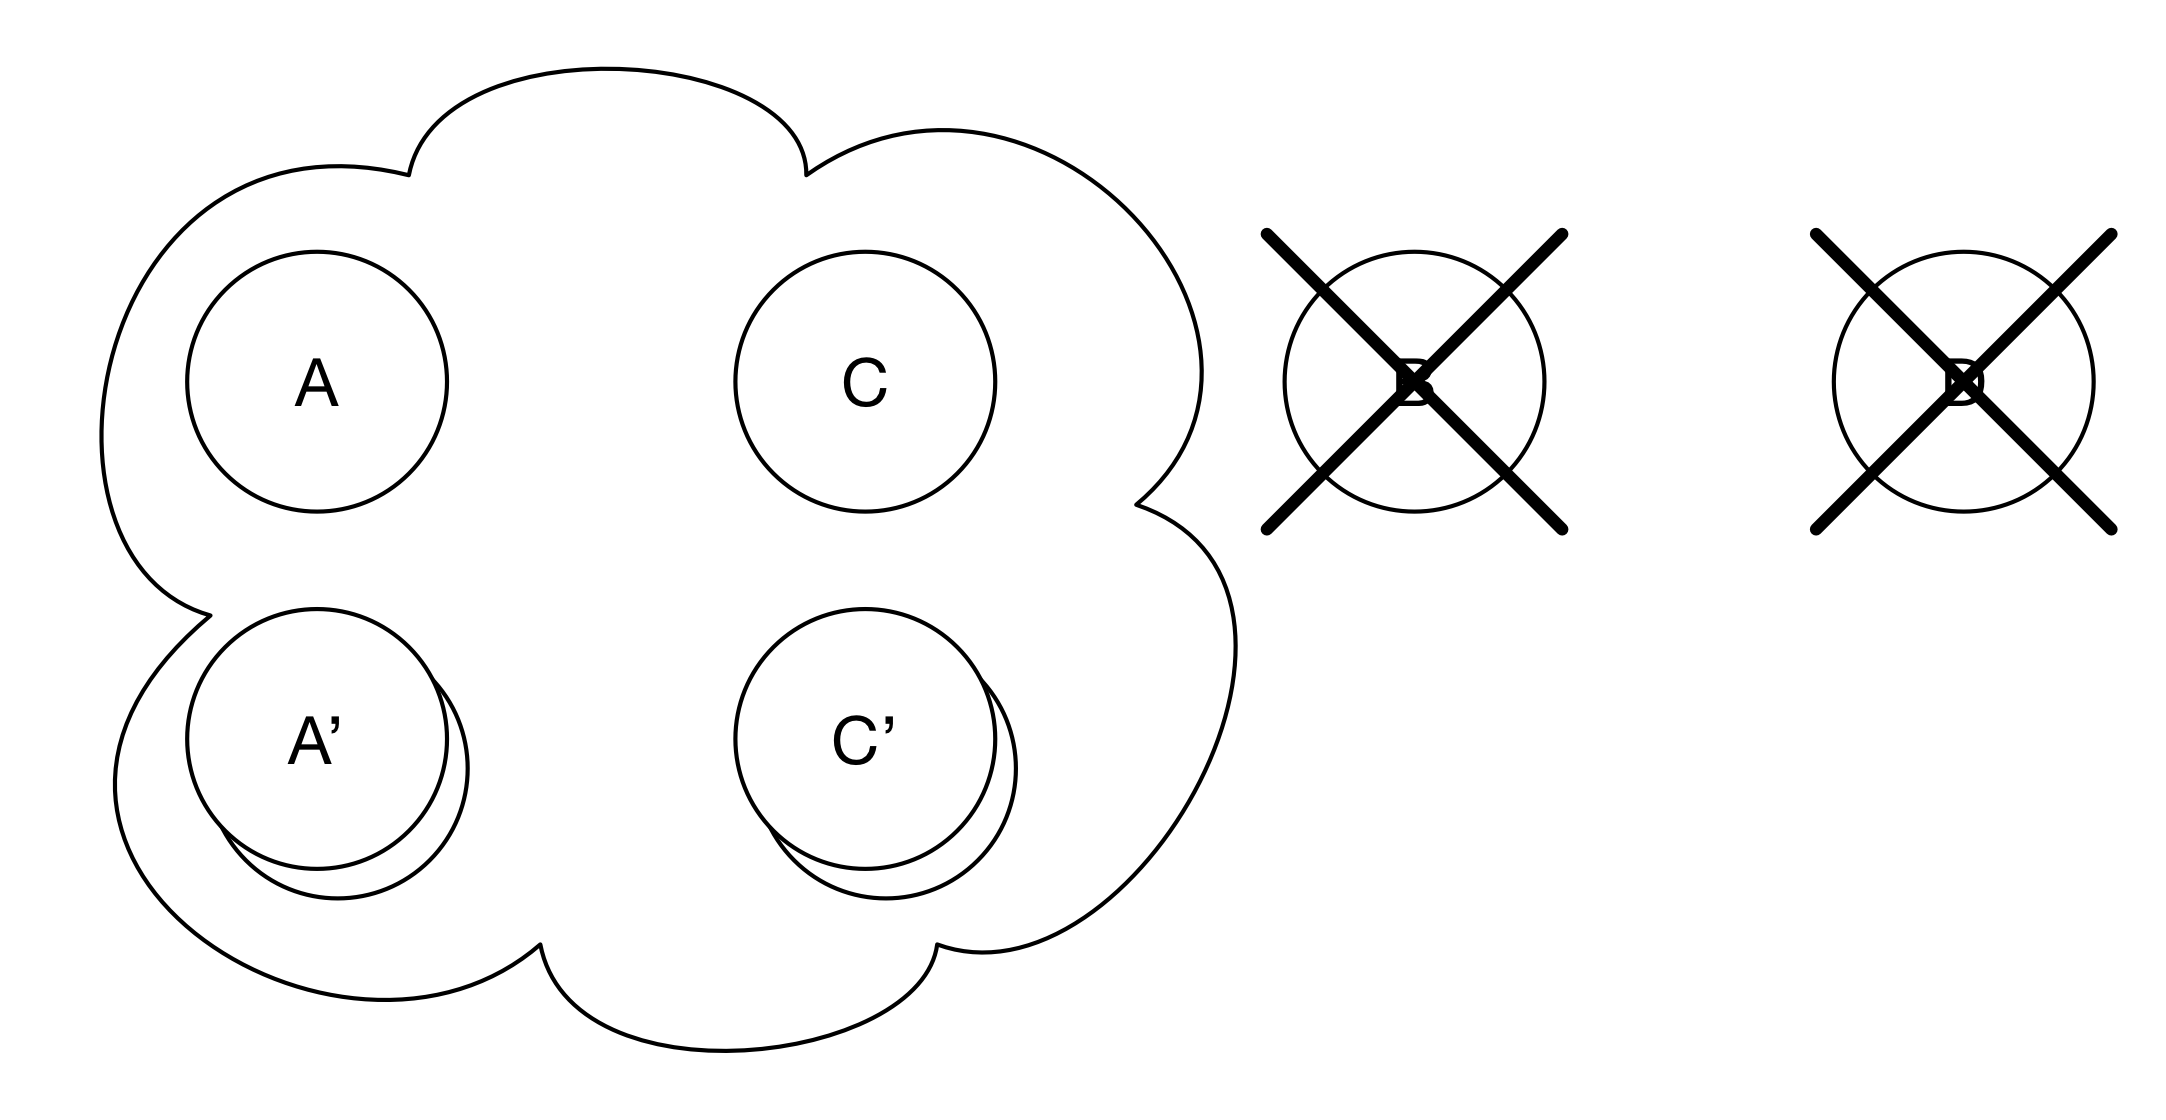
\includegraphics[width=7cm,keepaspectratio]{ri-model-sequence+location.png}
	\end{center}
\end{figure}

With the fine-grained location data available, the application is \emph{expecting} to see a movement that precedes exercises A or C. We call this movement the \emph{setup movement}. The setup movement classifier takes 1s of sensor input and produces probabilities classes that represent groups of exercises; this is particularly important for users that do not have a large number of sensors. If the user only wears an accelerometer on his or her wrist, then the setup movement for barbell bench press is the same as the setup movement for dumbbell bench press. In 94 \% of our test user base of 451, the next exercise prediction refined by the fine-grained location eliminated ambiguity of setup movement detection in all their exercises. \autoref{fig:model-sequence+setup} shows the final decision state of the mobile application.

\begin{figure}[hb]
	\begin{center}
		\caption{Exercise sequence model}
		\label{fig:model-sequence+setup}
		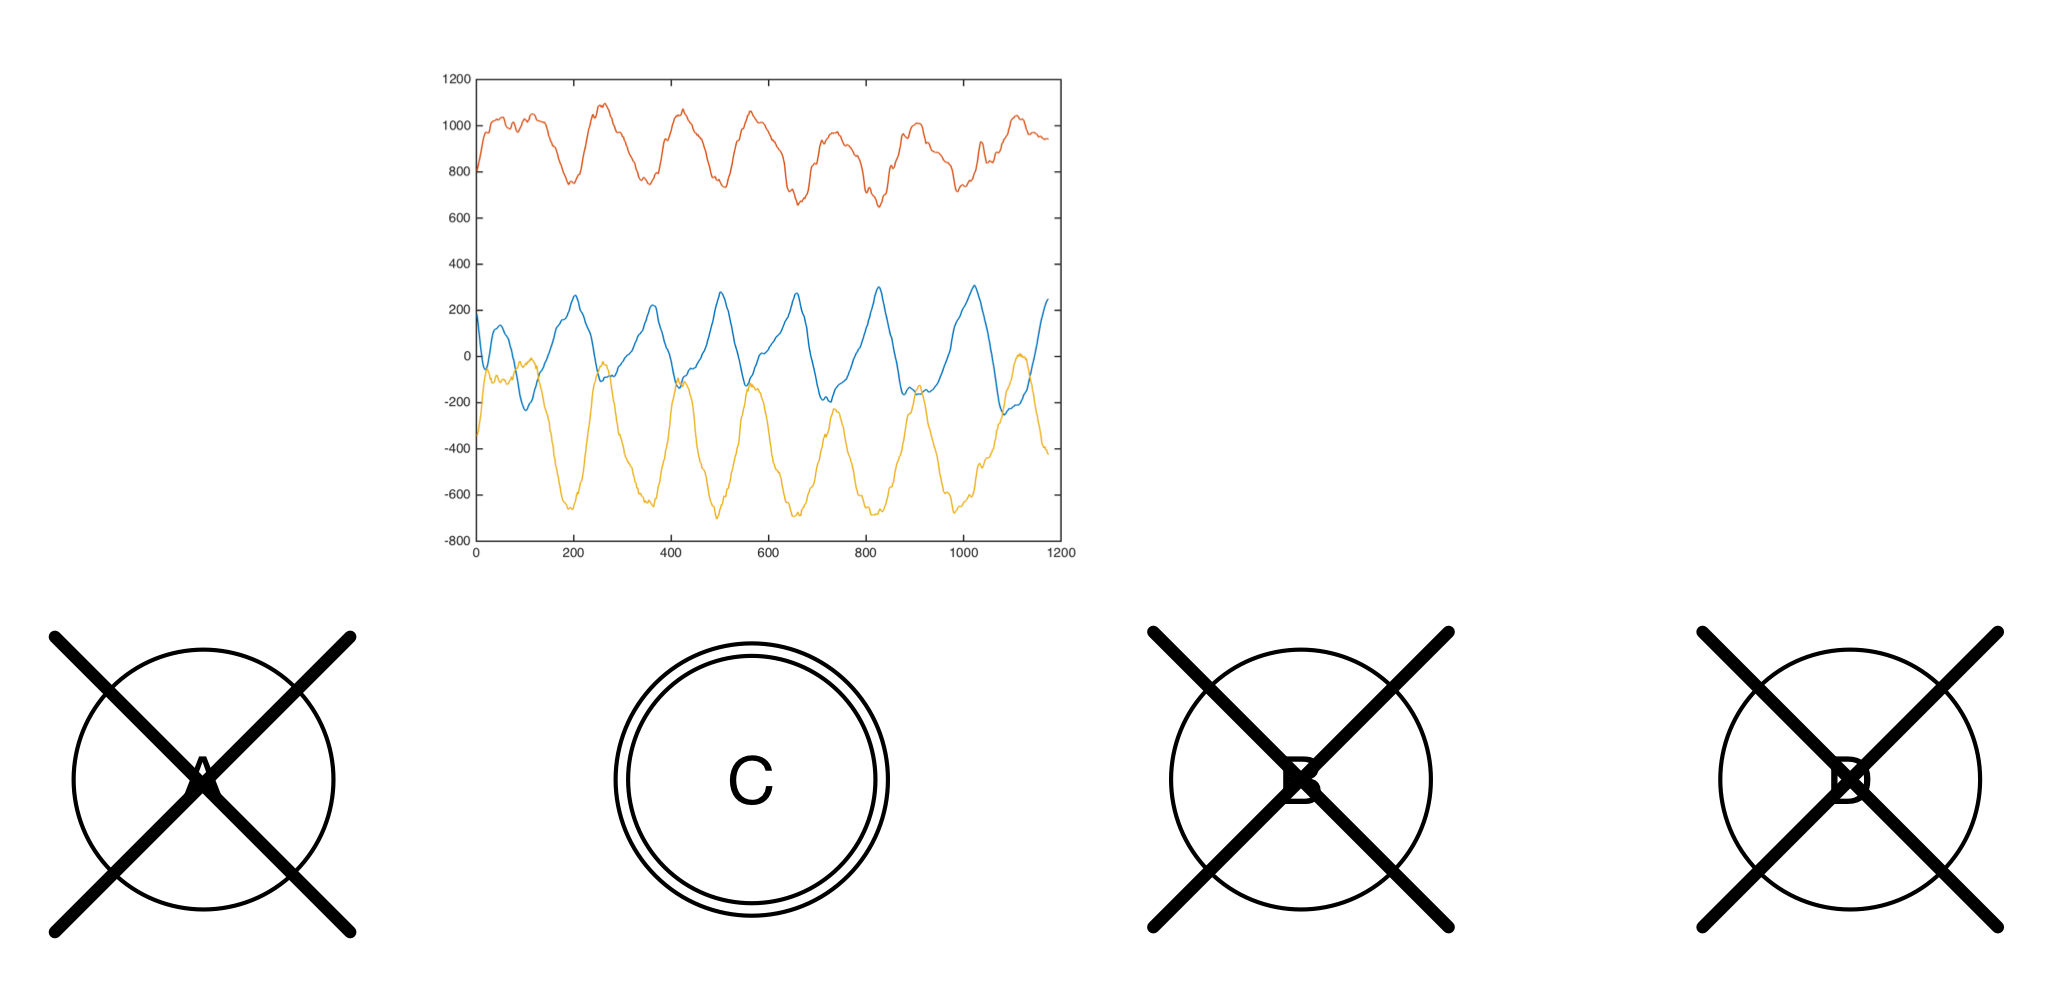
\includegraphics[width=7cm,keepaspectratio]{ri-model-sequence+setup.png}
	\end{center}
\end{figure}

\subsection{Sensor data}

The sensors send the data to the mobile application over BLE. The protocol as well as the hardware architecture of the devices places restrictions on the sample width and sampling rate. BLE protocol specifies maximum 80 bytes per message, and minimum duration of 7.5 ms between messages; this gives us theoretical maximum of 10640 bytes per second. With one particular hardware / firmware implementation, we found that the effective reliable data transfer rate drops to only 280 bytes per second. That particular device also lacked significant processing power. This gave us baseline protocol for 3-axis samples (such as acceleration or rotation), with 20 B for header and 5 B per sample. Packing the sample values into 40 bits gave us 3 $\times$ 13 bits and one bit for padding, and yielded code in \autoref{lst:threed-data}.

\begin{lstlisting}[language=C,caption={BLE 3-axis data},label={lst:threed-data}]
#define PACKED __attribute__((__packed__))

struct PACKED threed_data {
    int16_t x_val : 13;           // 13
    int16_t y_val : 13;           // 26
    int16_t z_val : 13;           // 39
    int16_t _     : 1;            // 40
};

struct PACKED header {
    uint16_t preamble;            // 2
    uint8_t types_count;          // 3
    uint8_t samples_per_second;   // 4
    double timestamp;             // 12
    uint32_t count;               // 16
    uint32_t type;                // 20
};
\end{lstlisting}

The \lstinline{preamble} is a marker sequence, which also allows for detection of endian-ness; though all sensor data-collecting devices we have encountered so far are big endian. The payload consisting of \lstinline{header} followed by 50 samples of \lstinline{threed_data} results in 270 Bs$^{-1}$ over the BLE connection. 

The sensor data in the mobile application is a set of vectors containing 1 second of sensor input data, normalised to a range of $\interval[open]{-1}{1}$ by using a maximum reasonable value for acceleration, rotation, strain and heart rate. (Looking at figure \autoref{raw-acceleration}, one might consider 4 ms$^{-2}$ to be such reasonable acceleration.) 

\begin{figure}[hp]
	\begin{center}
		\caption{Raw acceleration data}
		\label{raw-acceleration}
		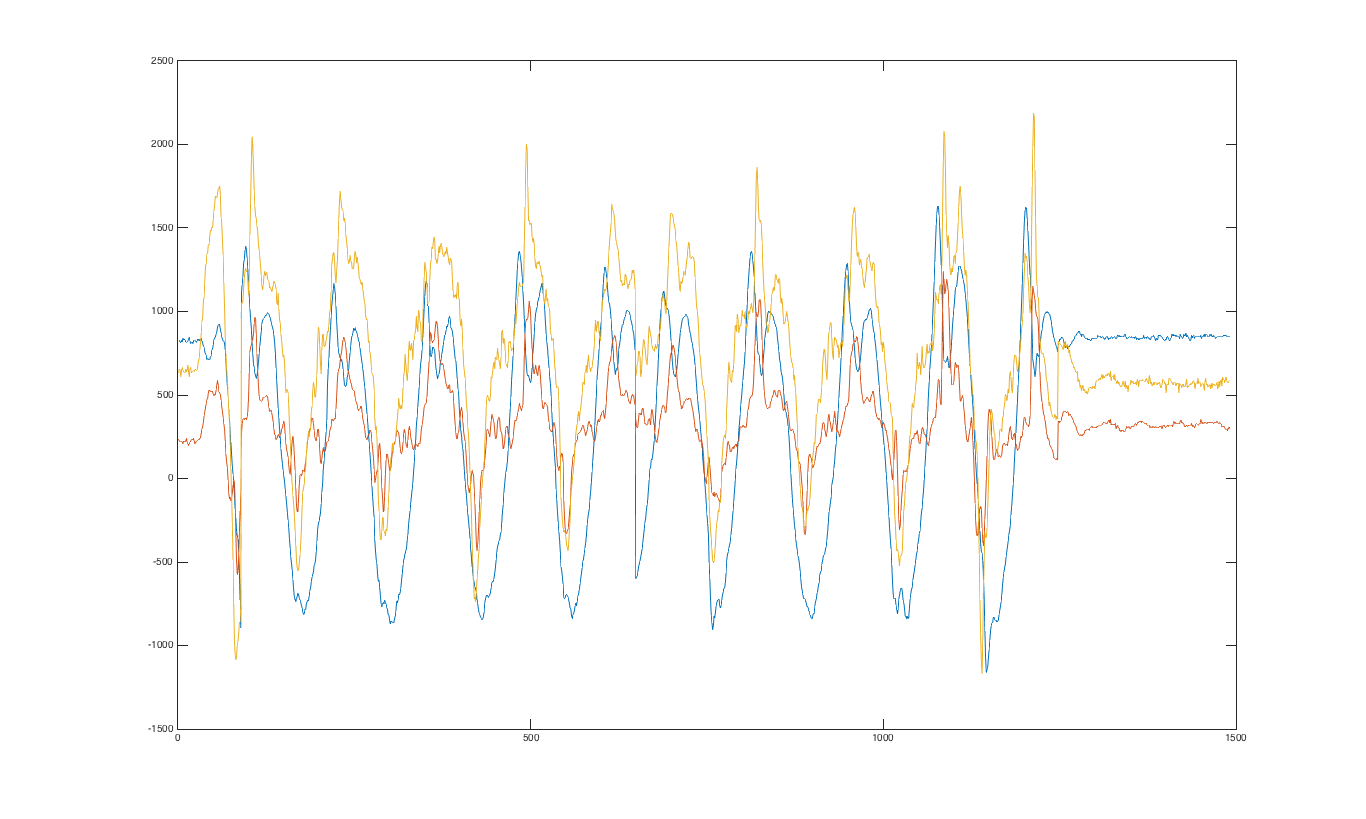
\includegraphics[width=7cm,keepaspectratio]{ri-raw-acceleration.png}
	\end{center}
\end{figure}


It is important to realise that a single sensor input alone is not sufficient to accurately distinguish exercise from non-exercise. 

\begin{table}[h]
\caption{Evaluation of a CNN for exercise vs. non-exercise classification}
\label{exercise}
\begin{center}
\begin{tabular}{|c||c||c|}
\hline
Actual / Predicted & Exercise & Non-exercise\\
\hline
Exercise & 12330 & 2305\\
\hline
Non-exercise & 3542 & 13412\\
\hline
\end{tabular}
\end{center}
\end{table}

\section{Summary}

TODO

\addtolength{\textheight}{-12cm}  % This command serves to balance the column lengths
                                  % on the last page of the document manually. It shortens
                                  % the textheight of the last page by a suitable amount.
                                  % This command does not take effect until the next page
                                  % so it should come on the page before the last. Make
                                  % sure that you do not shorten the textheight too much.

\begin{thebibliography}{99}

\bibitem{markov-chain-exercise} F. Oo, Q. Uux. Bar. 2016.
\bibitem{akka} Akka.
\bibitem{cqrs-es} CQRS/ES.
\bibitem{apache-cassandra} Apache Cassandra.
\bibitem{apache-spark} Apache Spark.
\bibitem{ibeacon} iBeacon.

\end{thebibliography}


\end{document}
